\documentclass[12pt]{article}
\usepackage{verbatim}
\usepackage{amsmath}
\usepackage{amssymb}
\usepackage{graphicx}
\usepackage[english]{babel}
\usepackage{caption}
\usepackage{subcaption}
\usepackage{ulem}

\usepackage{fullpage}
\usepackage{parskip}

\usepackage{amsmath,tikz}
\usetikzlibrary{shapes.geometric,arrows,positioning,calc}


%%% ------- New commands -------- %%%
\newcommand{\PoA}{\text{PoA}}

%%% ------- Game Pic ------- %%%%

\tikzstyle{player} = [draw, fill=red!80, shape=circle, minimum width=.25cm]
\tikzstyle{terminal} = [draw, shape = rectangle, fill=red!60, minimum width=.75cm, minimum height=.75cm]



%%% ------- Simulation ------- %%%%

\tikzstyle{Process} = [draw, shape = rectangle, fill=blue!20, minimum width=2.5cm, minimum height=1cm, text width=1.5cm,align=center]

\tikzstyle{Terminal} = [draw, fill=red!60,thick ,rectangle ,rounded corners, minimum width=3cm, minimum height=1cm]

\tikzstyle{Decision} = [draw, diamond ,minimum width=3.5cm, minimum height=1.5cm]

\tikzstyle{Result} = [draw , shape = rectangle, minimum width=1.5cm, minimum height=.8cm]

\tikzstyle{Arrow} = [->, >=latex', shorten >=1pt, thick]

\tikzstyle{left} = [draw, -latex',thick]


\title{Understanding the effect of selfish behaviour in a series of two queues.}
\author{Jason Young, Vincent Knight}


\begin{document}

When the cat goes: the paper is ready.

\begin{center}
  
\includegraphics[width=.5\textwidth]{Images/cat.jpg}
\end{center}

\maketitle

\begin{abstract}

Hierarchical queues in HC;
PoA;
Simulation model;
Heuristics developed to obtain optimal policies;

\end{abstract}

\section{Introduction}\label{Introduction}

Queues arise in a variety of settings: road traffic, data transfer and healthcare are just a few examples.
A large quantity of literature has investigated strategic decision making (for example: whether or not to join a queue) with regards to queues stemming from \cite{}.
When leaving one queue; customers (which we will refer to as players) often join a second queue and this is what is referred to as a hierarchical queueing system (as shown in Figure \ref{game_pic}).

There is a wide range of literature evidencing the negative effect of selfish actions in queueing systems \cite{}.
The following is a general conclusion of a majority of the literature:

\begin{quote}
Selfish users make busier systems.
\end{quote}

\begin{itemize}
    \item Naor;
    \item VK+PH;
    \item RS;
    \item Bell Stidham;
    \item Hassani book;
    \item Rouhgharden;
\end{itemize}

The effect of selfish behaviour when compared to optimal behaviour can be quantified as the Price of Anarchy (PoA).
This is defined as the ratio of the selfish ($\tilde C$) and optimal ($C^*$) costs:

$$
\PoA = \frac{\tilde C}{C^*}
$$

The contribution of this paper is to consider two stations (to avoid confusion we will refer to a queue and service station as a station) in series allowing for two consecutive decisions: whether or not to join the station.
Players who join the first station upon completion of service will potentially drop out from the entire system.
A potential application of this is a healthcare system where patients must choose to see their general practitioner before obtaining care from a specialist/emergency centre.

In Section \ref{model}, the model will be described.
A novel aspect of this work is that the cost of a given policy is evaluated through the use of purpose built Agent Based Simulation (ABS).
In Section \ref{heuristicoptimalpolicies} various heuristic approaches to obtaining optimal policies are considered.
These range from random search algorithms to a more sophisticated approach that depends on the analytical formula for an $M/M/c$ queue \cite{Stewart}.
Before concluding in Section \ref{conclusions} a variety of numerical experiments will be shown in Section \ref{results} demonstrating the effect of selfish decision making in queues in series.

\section{Model}\label{model}

Let $k\{1,2\}$ be the index for each station in the system.
The players arrive into the system at a rate $\Lambda$.
The players know the rate of service $\mu_k$ at each station, the number of servers at each station $c_k$ and also the number of players currently in each station.
Upon observing a station, players must select one of two potential strategies: `join' or `skip'.
The strategy picked at station $k$ is denoted by $d_k\in\{0,1\}$:

\begin{equation}\label{eq:decision}
    d_k=
\begin{cases}
    1,& \text{if player joins queue } k \\
    0,& \text{if player skips queue } k
\end{cases}
\end{equation}

The cost associated with joining system $k$ is denoted by $J_k$ and corresponds to the actual time spent in system $k$.
The cost associated with skipping station $k$ is denoted by $\beta_k$.
The cumulative cost of going through the entire system is given by $C=C(d)=C_1(d)+C_2(d)$ where:

\begin{equation}\label{eq:actualcost}
C_{k} = \begin{cases}
        \beta_k&\text{if }d_k=0\\
        J_k&\text{if }d_k=1\\
        \end{cases}
\end{equation}

The expected value of $J_k$ when there are $m$ players present upon arrival in system $k$ is given by:

\begin{equation} \label{eq:expect}
	E[J_{k}] = \frac{m+1}{\mu_k c_k}
\end{equation}

A final parameter of our model is the dropout probability $p$.
This is the probability with which a player who joins the first station will exit the entire system (implying $C_2=0$).

All of this is summarised in Figure \ref{game_pic}.

\begin{figure}[!hpbt]
\begin{center}
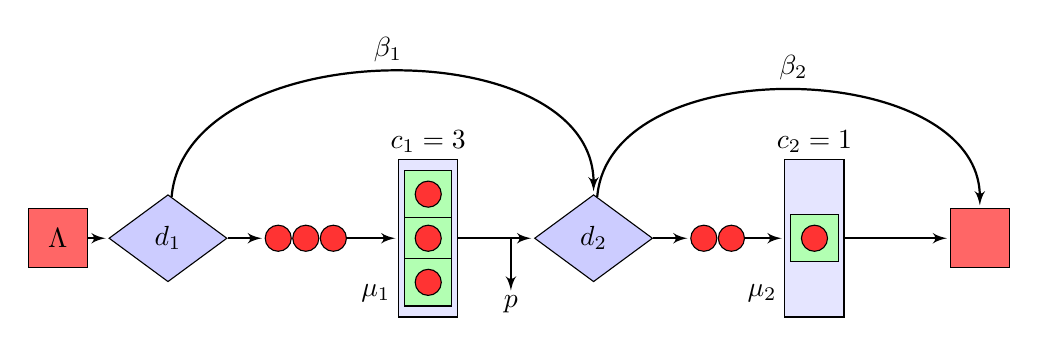
\begin{tikzpicture}[scale=.7]
            \draw (0,0) node[terminal] (A) {};
            \node (B) [diamond, fill=blue!20, draw, minimum width=1.5cm, minimum height=1cm] at (2, 0) {$d_1$};
            %%%%% First station %%%%%
            \draw (4,0) node[player] (C) {};
            \draw (4.5,0) node[player] (Q) {};
            \draw (5,0) node[player] (D) {};
            \draw [Arrow] (A) -- (B);
            \draw [Arrow] (B) -- (C);
            \node (E) [rectangle, fill=blue!10, draw, minimum width=.75cm, minimum height=2cm, right=1.0cm of Q] {};
            \draw [Arrow] (D) -- (E);
            \node (F) [rectangle, fill=green!30, draw, minimum width=.6cm, minimum height=.6cm] at (E) {};
            \node (G) [rectangle, fill=green!30, draw, minimum width=.6cm, minimum height=.6cm] at ($(E) + (0,.8)$) {};
            \node (H) [rectangle, fill=green!30, draw, minimum width=.6cm, minimum height=.6cm] at ($(E) + (0,-.8)$) {};
            \draw node[player] at (F) {};
            \draw node[player] at (G) {};
            \draw node[player] at (H) {};
            \node at ($(E) + (0,1.75)$) {$c_1=3$};
            \node at ($(E) + (-.95,-1)$) {$\mu_1$};
            %%%%% Second station %%%%%

            \node (Z) [diamond, fill=blue!20, draw, minimum width=1.5cm, minimum height=1cm] at ($(E) + (3,0)$) {$d_2$};

%            \node (R) [diamond, fill=blue!20, draw, minimum width=1.5cm, minimum height=1cm] at ($(Z) + (3,0)$) {$d_n$};
            \draw [Arrow] (E) -- (Z);
            \draw node[player] (I) at ($(Z) + (2,0)$) {};
            \draw node[player] (J) at ($(I) + (.5,0)$) {};
            \node (K) [rectangle, fill=blue!10, draw, minimum width=.75cm, minimum height=2cm, right=.5cm of J] {};
            \draw [Arrow] (Z) -- (I);
            \draw [Arrow] (J) -- (K);
            \node (L) [rectangle, fill=green!30, draw, minimum width=.6cm, minimum height=.6cm] at (K) {};
            \draw node[player] at (L) {};
            %%%%% End station %%%%
            \node (M) [terminal] at ($(K) + (3,0)$) {};
            \draw [Arrow] (K) -- (M);
            %%%%% Edges %%%%%
            \draw (Z) edge[out=85,in=90,Arrow] node [above] {$\beta_2$} (M);
            \draw (B) edge[out=85,in=90,Arrow] node [above] {$\beta_1$} (Z);
            \node at ($(K) + (0,1.75)$) {$c_2=1$};
            \node at ($(K) + (-.95,-1)$) {$\mu_2$};
            \node at (A) {$\Lambda$};

            %%%%% Dropout probability %%%%
            \draw ($(Z) !.5! (E)$) edge[Arrow] node [below = .25cm] {$p$} ($(Z) !.5! (E) + (0,-1)$);

        \end{tikzpicture}
    \end{center}

    \caption{Diagrammatic representation of the model.}
	\label{game_pic}

\end{figure}

If a general population of players is considered a state dependent policy $\tau = (n_1, n_2)$ can be defined that all players follow.
In general this policy will be of the form:

$$d_k = \begin{cases}
1,& \text{if }m_k\leq n_k\\
0,&\text{ otherwise}
\end{cases}$$

Where $m_k$ is the number of players present at station $k$ upon having to make a decision $d_k$.
In other words a policy $\tau$ is a set of two threshold policies, one for each station, simply denoting a threshold at which players skip.
As $d=d(\tau)$ we have $C=C(\tau)$.

DISCUSS SOLUTION SPACE FOR $\tau$: $\Omega$.

The optimal cost is thus defined as:

\begin{equation}\label{eq:optimal}
C^*=\min_{\tau\in\Omega}E[C(\tau)]
\end{equation}

Note that the restriction of the optimisation problem to only consider stationary policies is potentially an incorrect one.
Indeed, a non homogeneous policy could in fact be optimal however \textbf{FIND REFERENCE AND PAPER THAT SAYS THAT AN OPTIMAL POLICY WOULD BE HOMOGENOUS}.

The particular policy that gives $C^*$ will be denoted as $\tau^*$.
Another policy that will be considered in this paper is the selfish policy $\tilde\tau$.
The selfish policy is the policy under which individual players reduce their expected cost.

To obtain the selfish policy a further assumption is made: players are pessimistic.
It is assumed that players ignore the dropout probability $p$ at decision $d_1$ so that we have (recall equation (\ref{eq:decision})):

\begin{equation}\label{eq:selfishdecision}
    \tilde d_k=
\begin{cases}
    1,& \text{if } E[J_k] \leq \beta_k \\
    0,& \text{otherwise}
\end{cases}
\end{equation}

This in turn gives (recalling (\ref{eq:expect})):

\begin{equation}\label{eq:selfishpolicy}
\tilde\tau = \left(\lfloor\beta_1\mu_1 c_1 - 1\rfloor,\lfloor\beta_2\mu_2 c_2 - 1\rfloor\right)
\end{equation}

To evaluate the $C(\tau)$ for given $\tau$ a bespoke simulation model has been developed  (written in Python \cite{web001}).
The model itself is a combination of Discrete Event \cite{cite003} and Agent Based \cite{cite004} Simulation (taking advantage of the Object Orientated framework available in Python).
The flow of the simulation model is shown in Figure \ref{fig:Simflow}.

\begin{figure}[!hbpt]

        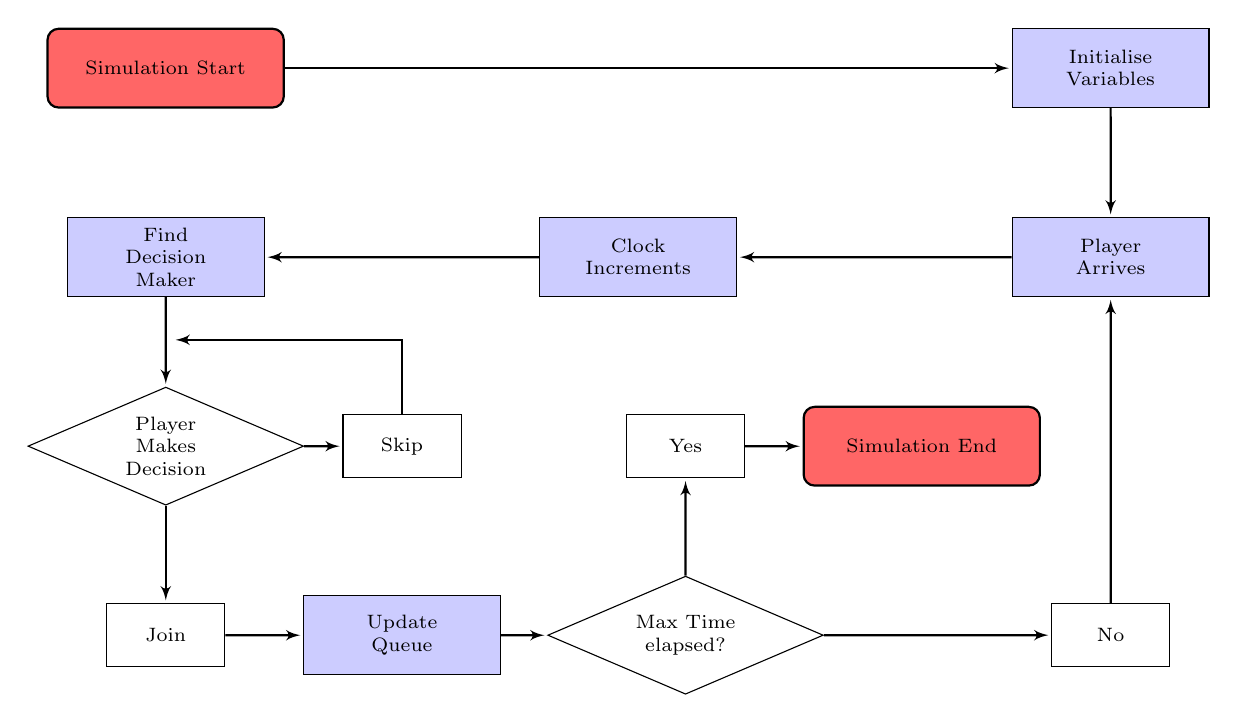
\begin{tikzpicture}[scale=.6]
        \tikzstyle{every node} = [font=\scriptsize ]

        %%%%% Top Line %%%%%%

        \draw (0,0) node[Terminal] (A) {Simulation Start};
        \draw node[Process] at ($(A)+ (20,0)$) (B) {Initialise Variables};


        %%%%% Second Line %%%%%

        \draw node[Process] at ($(B)+ (0,-4)$) (C){Player Arrives};
        \draw node[Process] at ($(C)+ (-10,0)$) (D){Clock Increments};
        \draw node[Process] at ($(D)+ (-10,0)$) (E){Find Decision Maker};

        %%%%% Third Line %%%%%

        \draw node[Decision] at ($(E) + (0,-4)$) (F){};
        \node[text width=1.5cm,align=center] at (F) {Player Makes  Decision};
        \draw node[Result] at ($(F) + (5,0)$) (G){Skip};
        \draw node[Result] at ($(G) + (6,0)$) (H){Yes};
        \draw node[Terminal] at ($(H) + (5,0)$) (I){Simulation End};

        %%%%% Bottom Line %%%%%

        \draw node[Result] at ($(F)+ (0,-4)$) (J){Join};
        \draw node[Process] at ($(J) + (5,0)$) (K){Update Queue};
        \draw node[Decision] at ($(H) + (0,-4)$) (L){};
        \node[text width=1.5cm,align=center] at (L) {Max Time elapsed?};
        \draw node[Result] at ($(C) + (0,-8)$) (M){No};

        %%%%% Connecting Arrows %%%%%

        \draw [Arrow] (A) -- (B);
        \draw [Arrow] (B) -- (C);
        \draw [Arrow] (C) -- (D);
        \draw [Arrow] (D) -- (E);
        \draw [Arrow] (E) -- (F);
        \draw [Arrow] (F) -- (J);
        \draw [Arrow] (J) -- (K);
        \draw [Arrow] (K) -- (L);
        \draw [Arrow] (L) -- (M);
        \draw [Arrow] (M) -- (C);
        \draw [Arrow] (F) -- (G);
        \draw [Arrow] (L) -- (H);
        \draw [Arrow] (H) -- (I);

        \node[draw=none,fill=none] at ($(E)+ (0,-1.75)$) (dummy){};

        \path [left] (G.north) |- (dummy.east);

	\end{tikzpicture}

	\caption{Flow chart describing the simulation model}
	\label{fig:Simflow}
\end{figure}

The input to the model (apart from the system parameters described in Section \ref{model}) is a policy $\tau$ and the required output is $C(\tau)$.
An investigation of run time, warm up time, and number of trials was carried out to ensure a reliable value of $C(\tau)$ is output \cite{cite013}.
Graphical methods were used for system parameters discussed in Section \ref{results} and are shown in Figure \ref{runtime}.

\begin{figure}[!hbtp]
    $$\begin{array}{ccc}
        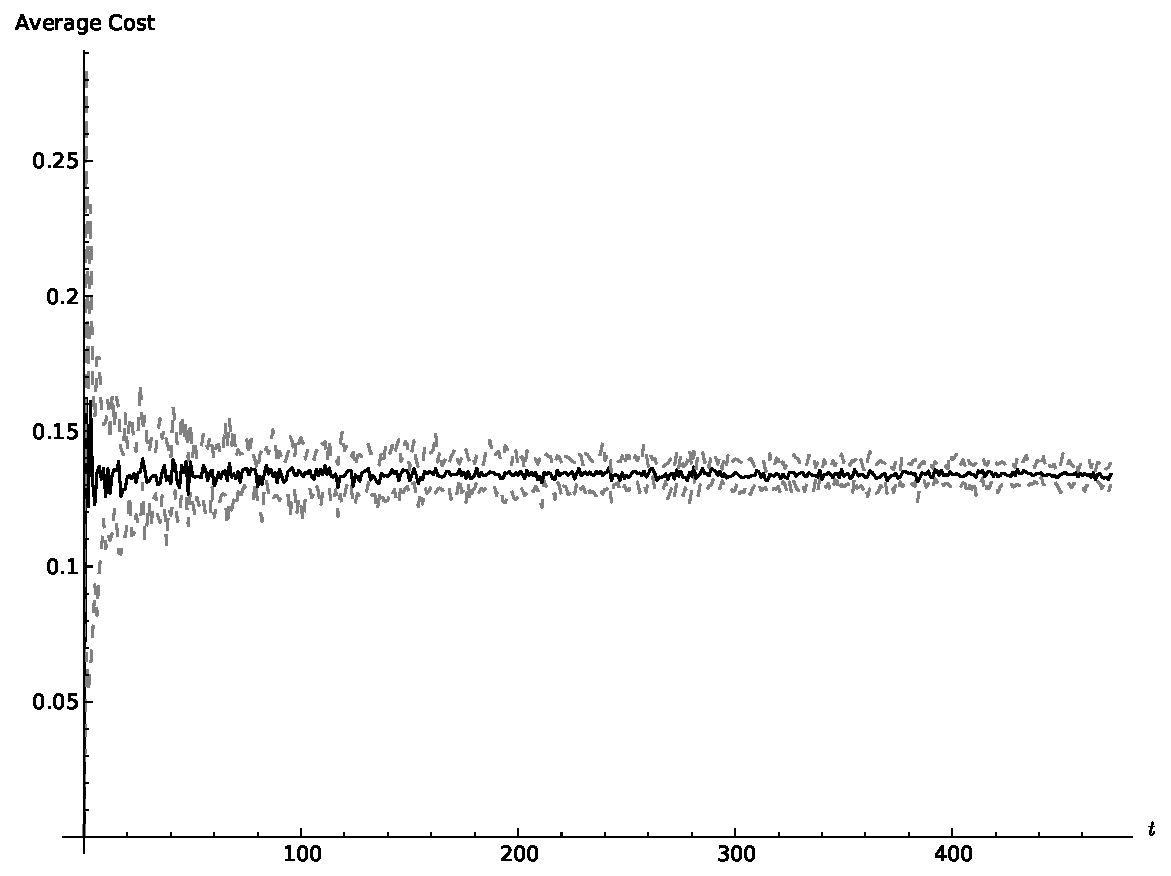
\includegraphics[width=.3\textwidth]{Images/Run_Time.pdf}&
        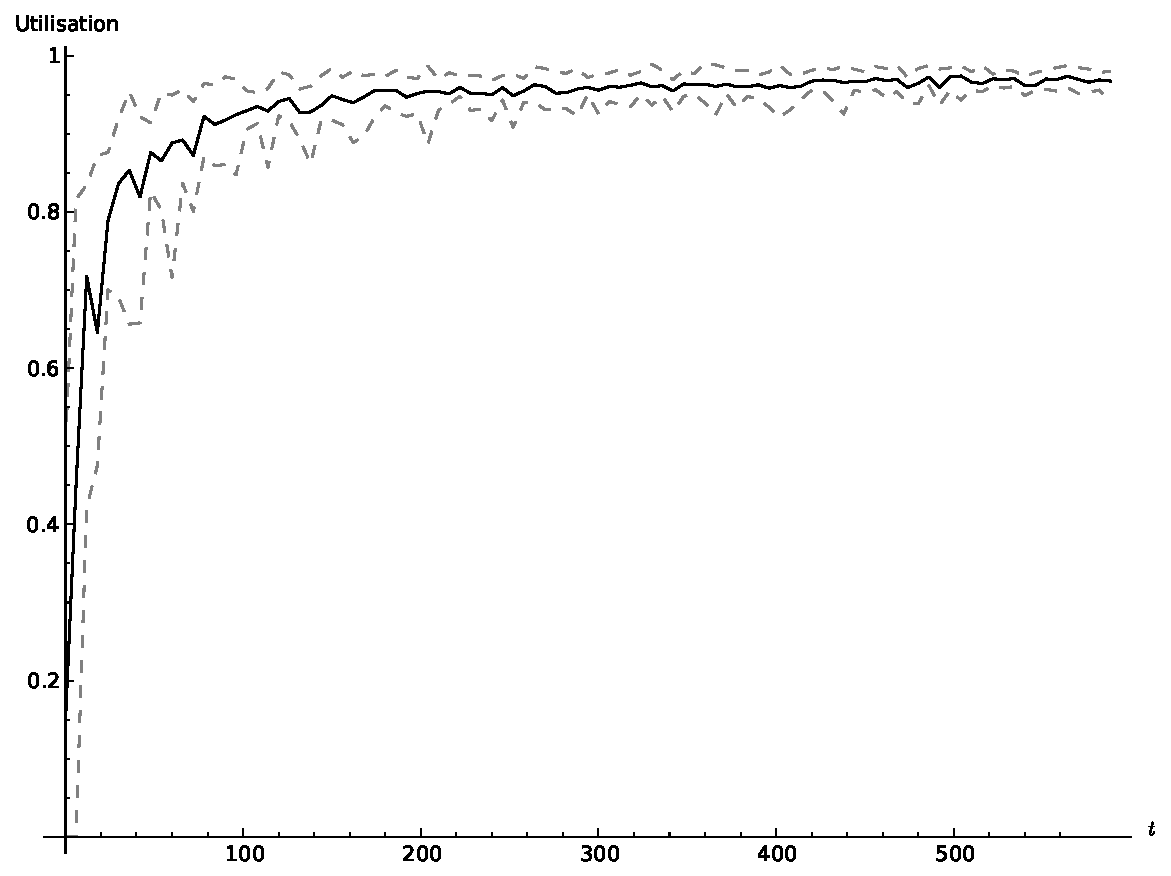
\includegraphics[width=.3\textwidth]{Images/Warm_up.pdf}&
        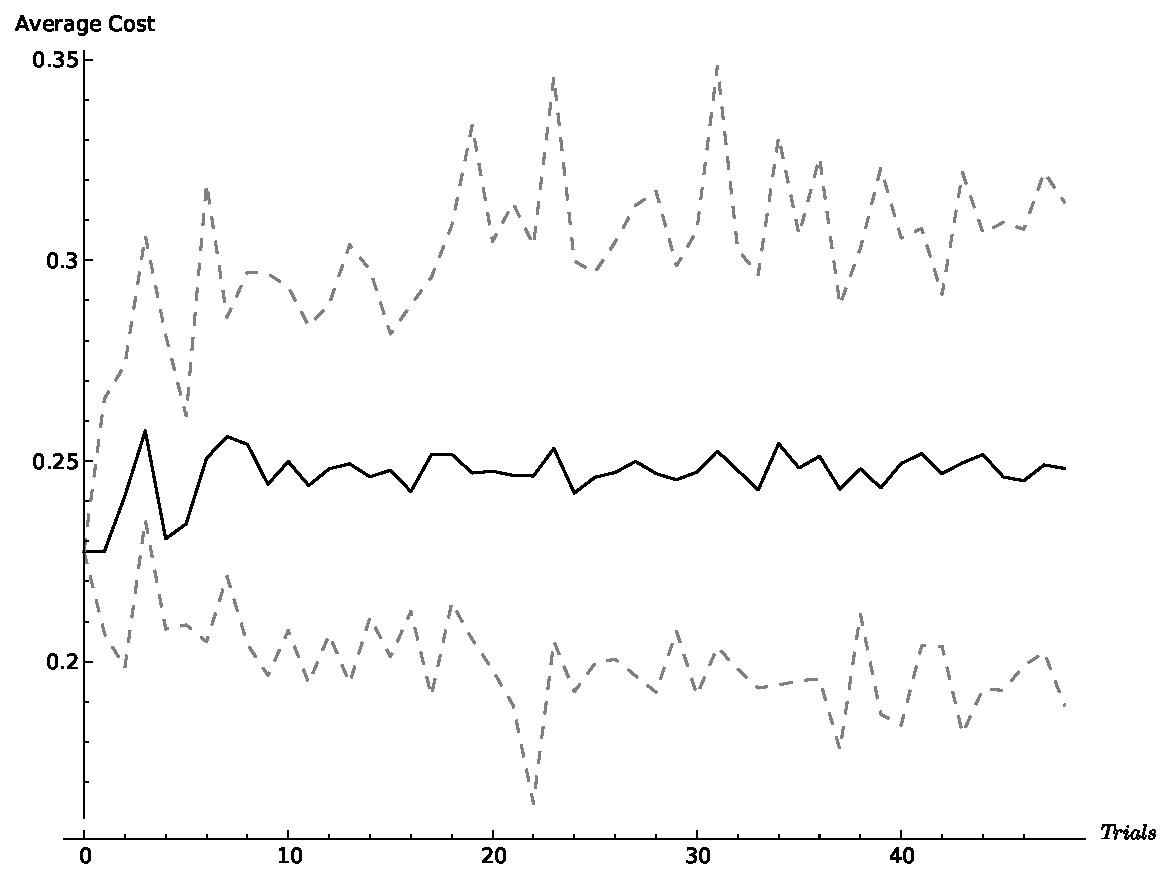
\includegraphics[width=.3\textwidth]{Images/Trials.pdf}\\
        \text{a: Run Time}& \text{b: Warm up time}& \text{c: Number of trials}
    \end{array}$$
    \caption{Investigating run time, warm up time and number of trials required to obtain reliable values of $C(\tau)$}\label{runtime}
\end{figure}

A run time of 250 time units was shown to reduce the variation in $C(\tau)$ (Figure \ref{runtime}a) whilst a warm up period of 50 time units reduced gave a stable utilisation of servers (Figure \ref{runtime}b).
Finally experiments of 16 trials each were chosen despite the lack of variation shown in Figure \ref{runtime}c.
This relatively large number of trials did not prove to be computationally expensive as they were all run in parallel using \ref{web002}.

As discussed, the simulation model is used as an objective function for a given $\tau$.
In the next section, various heuristic approaches to obtaining $\tau^*$ (recall (\ref{eq:optimal}): this corresponds to the optimal policy) will be discussed.

\section{Heuristic Optimal Policies}\label{heuristicoptimalpolicies}

Using the simulation model as an objective function a variety of search based heuristics have been tested \cite{}. All of these use $\tilde\tau$ as an initial solution and make minor perturbations accepting improvements within a specific region:

\begin{itemize}
    \item Fixed search range: randomly evaluate a fixed range around the initial policy;
    \item Variable search range: increase the range of the search range;
    \item Random descent: randomly search the entire solution space;
    \item Iterative random descent: JASON CHECK THESE AND ALSO INCLUDE A SENTENCE FOR THIS ONE. I DONT LIKE THE NAMES. ARE THEY THE CORRECT NAMES?
\end{itemize}

\subsection{Heuristic 1}\label{heuristic1}

A comparison of the performance of the various heuristics above is shown in Figure \ref{basicsearch}.

\begin{figure}[!hbtp]
    \begin{center}
        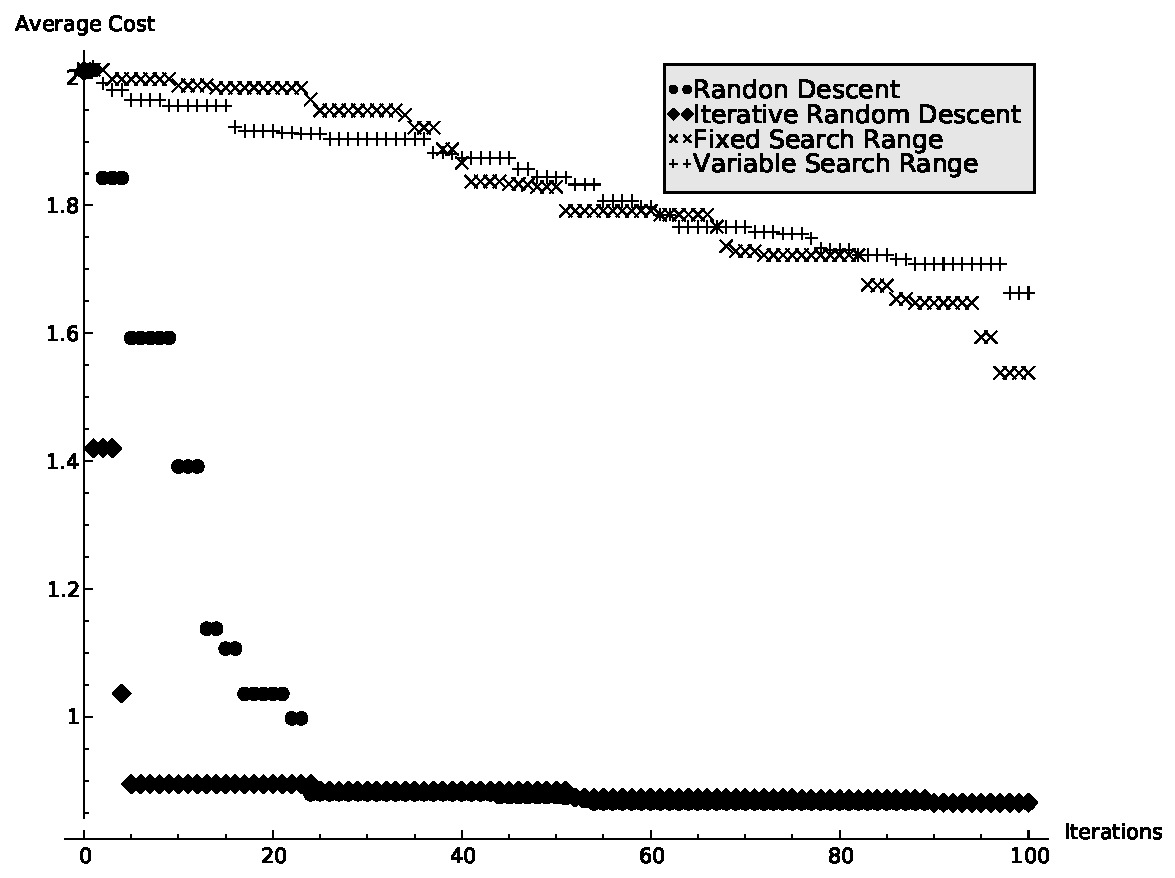
\includegraphics[width=.6\textwidth]{Images/Solver_Comp.pdf}
    \end{center}
    \caption{Comparing local search heuristics}\label{basicsearch}
\end{figure}

As shown, the most efficient of the chosen heuristics is the `Random Descent'.
This algorithm is nonetheless computationally expensive.
Some scenarios of Section \ref{results} taking various hours to run (despite the use of \cite{web002}).
The aim of the work presented here is to gain a global understanding of PoA behaviour and as such a large number of optimisations are needed.
The next sections will demonstrate further heuristics.

\subsection{Heuristic 2}\label{heuristic2}

This heuristic is based on the assumption that the arrival rate $\lambda_2$ at the second station is in fact Markovian.
For $p=0$ this is in fact not an assumption \ref{} however for $p>0$ the arrival rates at the second station no longer exhibit Markovian behaviour.
Nevertheless as shown in Figure \ref{casestudycomp} this heuristic performs very favourably and in fact the non Markovian behaviour seems to not affect the performance of our heuristic.

The arrival rate at the second station is given by:

\begin{equation}
\lambda_2 = \Lambda\times(1-p\times(1-\pi^{(1)}_{n_1}))
\end{equation}

Where $\tau=(n_1, n_2)$ and $\pi^{(1)}_{i}$ is the probability that the first station is in state $0\leq i\leq n_1$.
Note that the first station corresponds to an $M/M/c/n_1$ queue and so we have:

\begin{equation}\label{eq:probcl}
  \pi^{(1)}_i = \frac{1}{i!}\left(\frac{\Lambda}{\mu_1}\right)^{i}\pi_{0} \hspace{1cm} 0\leq i \leq c_i
\end{equation}

\begin{equation}\label{eq:probc_im}
  \pi^{(1)}_i = \frac{1}{c_i^{i-c_i}c_i!}\left(\frac{\Lambda}{\mu_1}\right)^{i}\pi_{0} \hspace{1cm} c_i< i \leq K
\end{equation}

where

\begin{equation}
\pi^{(1)}_{0} = \left[ \sum_{n=0}^{c_i-1} \frac{1}{n!} \left( \frac{\Lambda}{\mu_1} \right)^{n}  + \sum_{n=c_i}^{K} \frac{1}{c_i^{n-c_i}c_i!} \left( \frac{\Lambda}{\mu_1} \right)^{n} \right] ^{-1}
\end{equation}

Using the Markovian assumption as to the distribution of $\lambda_2$ a similar formula for $\pi_i^{(2)}$ can be obtained, replacing the relevant parameters.

Using this and recalling (\ref{actualcost}):

\begin{equation}\label{eq:ciapprox}
E[C_{i}] \approx \pi_{n_i}^{(i)} \beta_{i} + \sum_{j=0}^{c_{i}} \frac{\pi_{j}^{(i)}}{\mu_{i}} + \sum_{j=c_{i}}^{n_i-1}\frac{ \pi_{j}^{(i)}(j+1)}{ \mu_{i} c_{i}}
\end{equation}

and so:

\begin{equation}\label{eq:approxcost}
E[C]\approx E[C_1] + \frac{\lambda_2E[C_2]}{\Lambda}
\end{equation}

Note that the approximation of (\ref{eq:ciapprox}) is in fact an equality for $i=1$.
Using (\ref{eq:approxcost}) the cost of any policy $\tau$ can be approximated immediately and so $\tau^*$ can be heuristically obtained by an exhaustive search of the solution space.
To obtain an actual mean cost of $\tau^*$ the simulation model needs to only be run once.
A comparison of heuristics 1 and 2 is shown in Figure \ref{casestudycomp}, it is evident that the assumption made with regards to the Markovian nature of $\lambda_2$ do not seem to have a large effect.
The fact that results for $\Lambda >130$ are not shown for heuristic 1 are due to the fact that they were not obtained as they required more than 80 hours of computations on \cite{web002}.

\begin{figure}[!hbtp]
    \begin{center}
        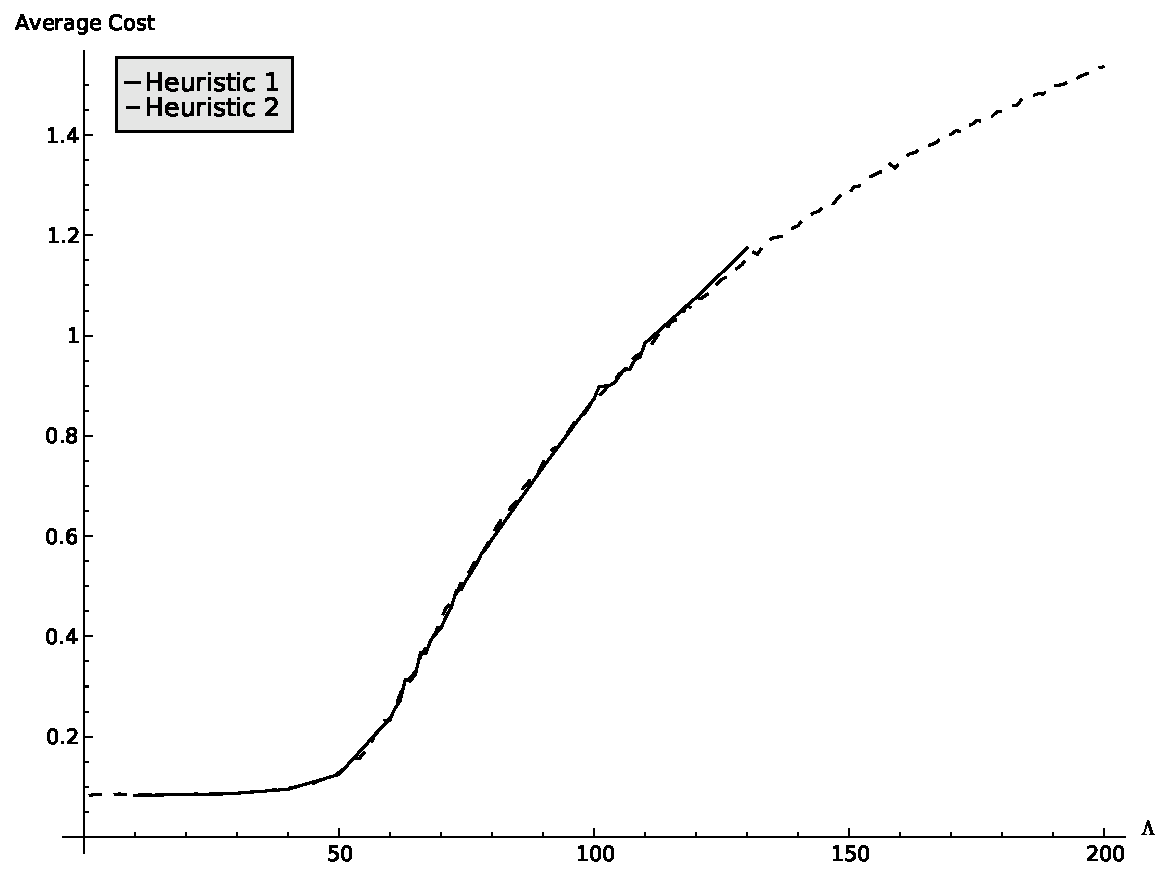
\includegraphics[width=.6\textwidth]{Images/CaseStudyComp.pdf}
    \end{center}
    \caption{Comparing Heuristic 1 and 2}\label{casestudycomp}
\end{figure}

Before considering various results in Section \ref{results}, one final heuristic is proposed that only applies if $c_1=c_2=1$.

\subsection{Heuristic 3}\label{heuristic3}

In \cite{Naor} thresholds $n^*$ are obtained for single server queues that optimise the expected cost. $n^*$ is shown to be the solution to the following inequality:

\begin{equation}\label{eq:naor}
  \leq  n ^ * \leq
\end{equation}

Using (\ref{eq:naor}) another potential policy is $\tau = (n^*_1, n^*_2)$.
Figure \ref{allheuristics} shows a comparison of these three heuristic approaches for a series of single server queues.

\begin{figure}[!hbtp]
    \begin{center}
        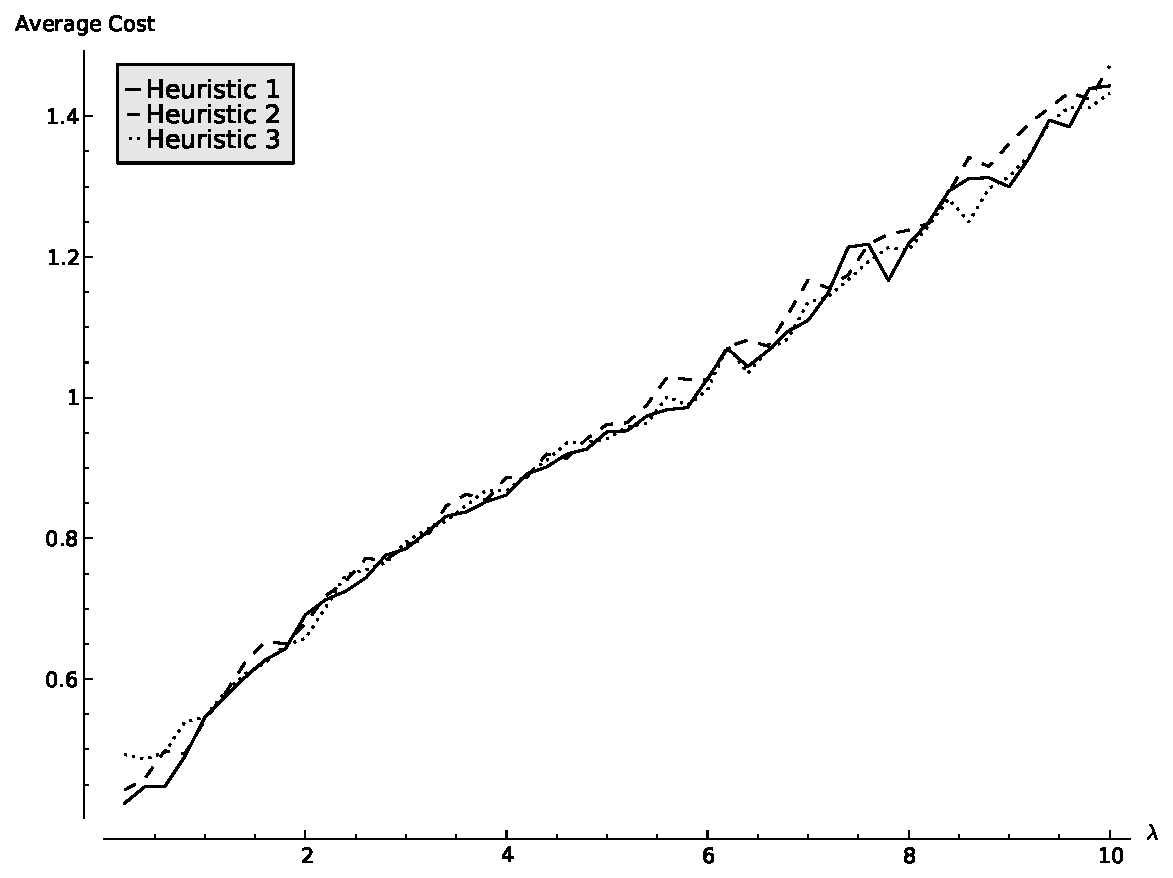
\includegraphics[width=.6\textwidth]{Images/Exit0.pdf}
    \end{center}
    \caption{Comparing all heuristics}\label{allheuristics}
\end{figure}

All the heuristics seem to behave adequately (this has been confirmed through a large quantity of experimentation).
For the purposes of this paper heuristic 2 will be used from now on given the very low computational cost.

\section{Results}\label{results}

As discussed in Section \label{introduction} an immediate application of the models developed is healthcare.
Using data from \cite{} we consider two stations in series:

\begin{itemize}
    \item A General practitioner with 5 servers each able to see 12.5 patients a day. Furthermore patients consider a wait of 2 days as acceptable to see their GP:

        $$c_1=5, \mu_1=12.5, \beta_1=2$$

    \item After seeing a GP or after deciding the wait to see a GP is too long \cite{FINDSOMEPOPNEWSABOUTTHIS} patients may choose to proceed to the Emergency Department (ED). It is assumed that the ED has a capacity of 5 servers each able to 2 patients an hour. An acceptable wait is now assumed to be 8 hours which is in line with national targets \cite{}.

        $$c_2=5, \mu_1=48, \beta_1=1/3$$
\end{itemize}

It is assumed that 80\% of patients who see their GP do not need to attend the ED:

$$p=.8$$

For these sets of parameters, using heuristic 2 a Price of Anarchy can be calculated.
For example for $\Lambda=?$ the PoA is 5 which implies that the overall patient utility is 5 times as bad when patients act selfishly.

Figure \ref{ana_lambda} shows the effect of $\Lambda$ on the PoA for different values of service ($\beta$).
The profile of this curve is very similar to profiles of curves seen in \cite{VKPH}.
For low demand the PoA is 1: this implies that the capacity of the system is sufficient to deal with the actions of selfish users.
As the demand increases, the first station starts to get congested.
Optimal behaviour will at this point encourage players to skip the first queue (before the expected wait reaches $\beta_1$.
Selfish users however will wait until the system becomes very busy before they are willing to start skipping.
This occurs when the demand increases further and we see an initial drop of the PoA.
Recall that this simply implies that selfish users are not causing the system to behave in a different way to the optimal behaviour.
This is something that has been noted in the literature: \cite{bunchofpapers}: in congested systems selfish users don't make a difference.
This is particularly relevant to healthcare where most healthcare systems are already severely over congested.

\begin{figure}[!hbtp]
    \begin{center}
        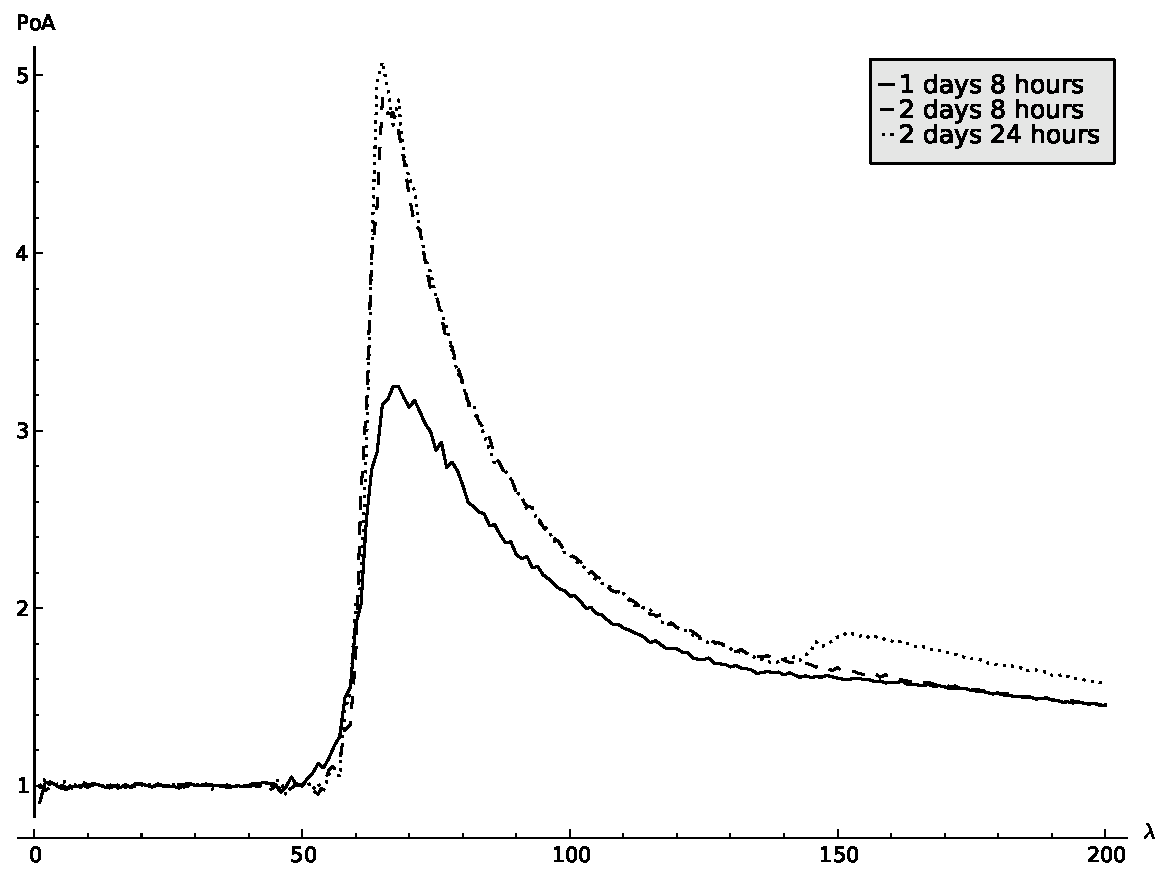
\includegraphics[width=.5\textwidth]{Images/Ana_Lambda.pdf}
    \end{center}
    \caption{PoA for varying lambda}\label{ana_lambda}
\end{figure}

As previously mention, increasing the length that patients are willing to wait causes the PoA increases
 which can be seen in Fig. \ref{fig:Demandparam}. Also interesting to note is the appearance of a second peak can be seen as the value of service at the A\&E increases.

\begin{figure}[!hbtp]
    \begin{center}
        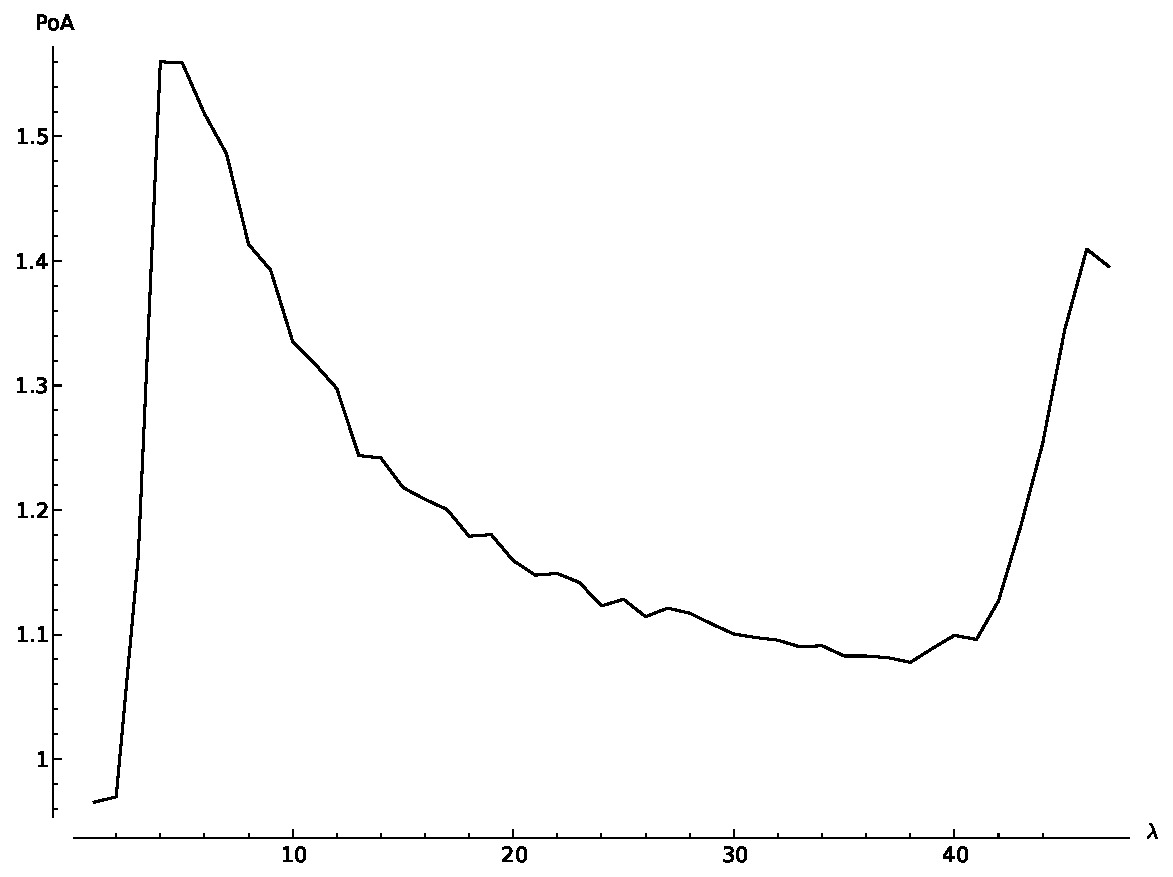
\includegraphics[width=.6\textwidth]{Images/DualPeak.pdf}
    \end{center}
    \caption{Another set of scenarios}\label{dualpeak}
\end{figure}

\section{Conclusions and Further work}\label{conclusions}

We can see in Fig.\ref{fig:EXTparam} (where we are modeling the above system), there does exist a dropout probability the minimises the negative impact due to choice. However in the practical situation of sending 85\% (Fig.\ref{fig:EXTparam}) of patients to an A\&E, it may not be feasible to implement this dropout probability.

\begin{figure}[!hbtp]
    \begin{center}
        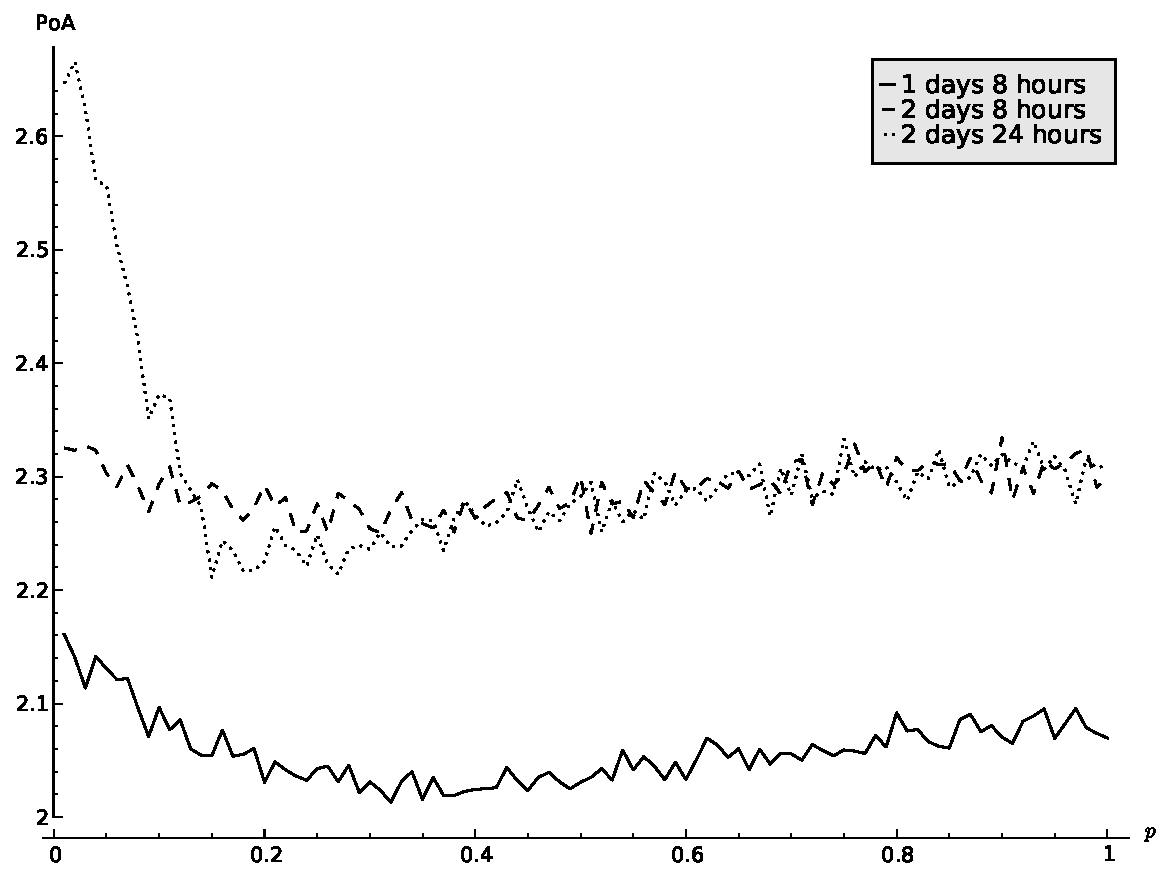
\includegraphics[width=.6\textwidth]{Images/AnaExit.pdf}
    \end{center}
    \caption{PoA for varying exit prob}\label{anaexit}
\end{figure}

\end{document}

% Starting from scratch, your stuff is below.

\begin{abstract}

In this paper, we consider a system consisting of $M/M/C$ queues arranged in series. When customers (referred to as players) arrive at a given queue as they move through the system, they make a decision, to either join the queue or skip it at a cost. The system is considered under two types of player behaviour, one where players act selfishly and one where there is a policy dictating the decisions of the players. Players acting selfishly will attempt to reduce their own cost with no thought to the cost of other players in the system. Alternatively a optimal social policy is considered that attempts to reduce the average cost per player. We use the Price of Anarchy as a measure of the inefficiency due to choice to observe the impact that individual behavior has on the system. An Agent Based Simulation is developed that is used in conjunction with various heuristic approaches to obtain the socially optimal and selfish behavior of players. Due to the high computational cost of this model an analytical approximation is obtained and used to identify the effect of the total arrival rate on the system as well as other system parameters. In particular an optimal dropout probability rate is obtained for various scenarios which could have applications such as the optimal referral rate of general practitioners to hierarchical medical services.

\end{abstract}

\section{Introduction}\label{Introduction}

\begin{itemize}
    \item Hierarchy in real life queues;
    \item Review of papers in BQT;
    \item PoA;
    \item Discussion of situation being modelled in this paper.
\end{itemize}

Consider a system where players within this system will act for their own good, attempting to reduce their cost or equivalently increase their utility. This work will quantify the impact that this choice has in hierarchical queueing systems.
In this paper and without loss of generality, cost is considered to be a unit-less combination of time spent in the system and any utility lost by balking from a given queue. It is well understood that individual behaviour has a negative effect on the efficiency of queueing systems.

To illustrate this effect, consider the classic game theory problem, the Prisoners Dilemma. The game is that two prisoners are being separately questioned and must decide whether to co-operate, or defect, and the cost to each player can be seen in Fig.\ref{fig:prisoner} . Under selfish conditions, both players defect, giving a cost per player of 5. However, if both players co-operate, the average cost per player is reduced to 1.

\begin{center}
  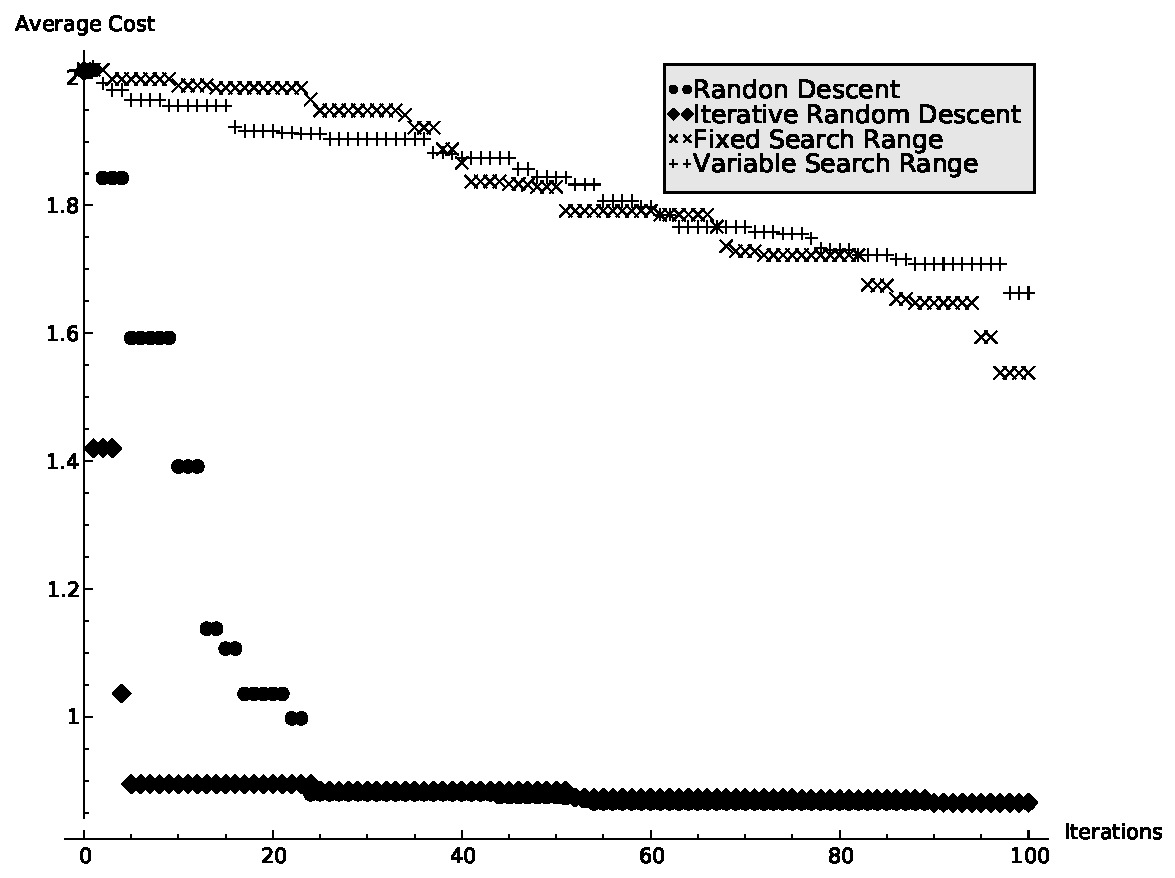
\includegraphics[width=.5\textwidth]{Images/Solver_Comp.pdf}
\end{center}


\begin{figure}[ht]
  \begin{center}

    \begin{tabular}{  c | c |c |}

      \cline{2-3}           & Co-operate & Defect 			 \\ \hline
      \multicolumn{1}{ |c| }{Co-operate} & (1,1)      & (7,0)   		 \\ \hline
      \multicolumn{1}{ |c| }{Defect}     & (0,7)      & (5,5)			 \\ \hline
    \end{tabular}

    \caption{Payoff matrix for a prisoners dilemma game}
    \label{fig:prisoner}
  \end{center}
\end{figure}




In \cite{cite002} Bell and Stidham look into a particular system where the queues were arranged in parrallel. Players knew the service time at each of these queues and could join any of them and recieve the same service. However players were not able to see the length of the queue before joining. This is an example of an unobservable queueing system, where players are not able to see the number of other players ahead of them prior to joining. Some work has been done in showing the differences in player behaviour in unobservable and observable versions of the same queue in \cite{cite010}. In that paper, the effect of the amount of information available to players, including some ``intentional vagueness" was studied while the system was under both selfish and social conditions.
Boudali \cite{cite011} studied the effect of choice in a system where there was a possibility of a catastrophe occurring and players would have to abandon the system, wasting the time spent waiting.


\section{Model}\label{model}

In this paper we will focus on a hierarchical queueing system in which players must progress through a series of queues as seen in Fig.\ref{fig:game_pic}.

\begin{figure}[ht]
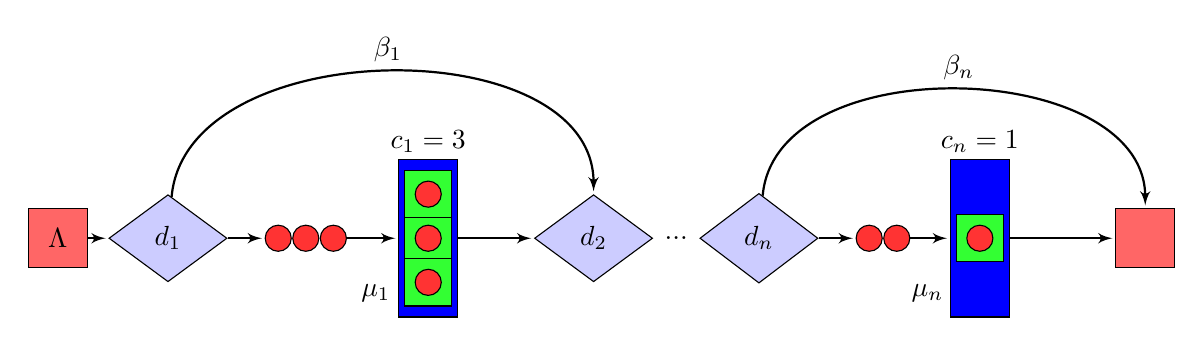
\begin{tikzpicture}[scale=.7]
            \draw (0,0) node[terminal] (A) {};
            \node (B) [diamond, fill=blue!20, draw, minimum width=1.5cm, minimum height=1cm] at (2, 0) {$d_1$};
            %%%%% First station %%%%%
            \draw (4,0) node[player] (C) {};
            \draw (4.5,0) node[player] (Q) {};
            \draw (5,0) node[player] (D) {};
            \draw [Arrow] (A) -- (B);
            \draw [Arrow] (B) -- (C);
            \node (E) [rectangle, fill=blue!100, draw, minimum width=.75cm, minimum height=2cm, right=1.0cm of Q] {};
            \draw [Arrow] (D) -- (E);
            \node (F) [rectangle, fill=green!80, draw, minimum width=.6cm, minimum height=.6cm] at (E) {};
            \node (G) [rectangle, fill=green!80, draw, minimum width=.6cm, minimum height=.6cm] at ($(E) + (0,.8)$) {};
            \node (H) [rectangle, fill=green!80, draw, minimum width=.6cm, minimum height=.6cm] at ($(E) + (0,-.8)$) {};
            \draw node[player] at (F) {};
            \draw node[player] at (G) {};
            \draw node[player] at (H) {};
            \node at ($(E) + (0,1.75)$) {$c_1=3$};
            \node at ($(E) + (-.95,-1)$) {$\mu_1$};
            %%%%% Second station %%%%%

            \node (Z) [diamond, fill=blue!20, draw, minimum width=1.5cm, minimum height=1cm] at ($(E) + (3,0)$) {$d_2$};

            \node (R) [diamond, fill=blue!20, draw, minimum width=1.5cm, minimum height=1cm] at ($(Z) + (3,0)$) {$d_n$};
            \draw [Arrow] (E) -- (Z);
            \draw node[player] (I) at ($(R) + (2,0)$) {};
            \draw node[player] (J) at ($(I) + (.5,0)$) {};
            \node (K) [rectangle, fill=blue!100, draw, minimum width=.75cm, minimum height=2cm, right=.5cm of J] {};
            \draw [Arrow] (R) -- (I);
            \draw [Arrow] (J) -- (K);
            \node (L) [rectangle, fill=green!80, draw, minimum width=.6cm, minimum height=.6cm] at (K) {};
            \draw node[player] at (L) {};
            %%%%% End station %%%%
            \node (M) [terminal] at ($(K) + (3,0)$) {};
            \draw [Arrow] (K) -- (M);
            %%%%% Edges %%%%%
            \draw (R) edge[out=85,in=90,Arrow] node [above] {$\beta_n$} (M);
            \draw (B) edge[out=85,in=90,Arrow] node [above] {$\beta_1$} (Z);
            \node at ($(K) + (0,1.75)$) {$c_n=1$};
            \node at ($(K) + (-.95,-1)$) {$\mu_n$};
            \node at (A) {$\Lambda$};

            %%%%% My bit %%%%%

            \node[draw=none,fill=none] at ($(Z)+ (1.5,0)$) {...};

        \end{tikzpicture}

    \caption{Diagram of n stations in series}
	\label{fig:game_pic}

\end{figure}

The players arrive into the system at a rate $\Lambda$ and make a decision on whether or not to join the first queue. The players know the rate of service $\mu_k$ at each queue , the number of servers at each queue $c_k$ and also the number of players currently in each queue. Once they observe a queue, they must either join the queue or skip the queue. There is a cost associated with skipping a particular queue give by $\beta_k$ .  There is also a chance that after completing service at a queue, the player would leave the system completely, known as the dropout probability $p_k$. Players make their decision $d_k$ by comparing the skipping cost to the expected cost of joining the queue .

\begin{equation}\label{eq:decision}
    d_k=
\begin{cases}
    1,& \text{if player joins queue } k \\
    0,& \text{if player skips queue } k
\end{cases}
\end{equation}

A player arriving at queue $k$ and observing $m$ agents ahead of them will expect to receive a cost given by equation (\ref{eq:expect}).

\begin{equation} \label{eq:expect}
	E[\sigma_{k}] = \frac{m+1}{\mu_k c_k}
\end{equation}

Where $\sigma_{k}$ denotes the actual cost to a player at station k.

In addition, we let $\xi$ denote the cumulative cost incurred by a player moving through the system. $T_{k}$ in eq \ref{eq:actualcost} denotes the actual time spent in station $k$ by a player. It is the sum of the time spent waiting to be served ($T^{w}_{k}$) and the time spent being served ($T^{s}_{k}$). Thus we have the cumulative cost to a player in station

\begin{equation}\label{eq:actualcost}
\xi_{k} = \begin{cases}
		0, \text{ if } i = 0 \\
        \xi_{k-1} + \begin{cases}
        	  	T_{k},& \text{if player joins queue k} \\
    			\beta_{k},& \text{if player skips queue k}
        	  \end{cases}

	  \end{cases}
\end{equation}

Upon arriving at queue $k$ a player will make a decision that will benefit them by comparing (\ref{eq:expect}) to $\beta_k$. For example, a player arriving at a queue with the parameters listed in Fig.\ref{fig:param} will expect to add .5 to their cost if they receive service at that station. As the balking cost for this queue is lower than the expected cost ($\beta=0.4$), this player would skip under selfish conditions.

\begin{figure}[ht]
  \begin{center}

    \begin{tabular}{ |l |r |}
                   			\hline
      Parameter  & Value \\ \hline
      $\mu$  & 2   		 \\ \hline
      $c$  & 4 			 \\ \hline
      $m$  & 3 			 \\ \hline
      $\beta$  & 0.4 	 \\ \hline
    \end{tabular}

    \caption{Example parameters for a station}
    \label{fig:param}
  \end{center}
\end{figure}

A player moving through the system with $n$ stations can expect to receive a cost of (\ref{eq:total}) when making a choice $d_k$(\ref{eq:decision}) at queue $k$ .




\begin{equation}\label{eq:total}
E[\xi_n] = \sum_{i=1}^{n}{(1-d_i)\left(\frac{m_i+1}{\mu_ic_i}\right)} + \sum_{i=1}^{n}{d_i\beta_i}
\end{equation}

% We want to write down a policy. That all players should follow. This will then give a mean cost for all players. This is what is implied by a social policy...
We want to instigate a policy which minimises the average cost per player, which is known as the optimal social policy. In the system, the policy is the length of the queue at which a player arriving at the queue will balk from it. Now consider Fig.\ref{fig:param}, and we can see that a player skips from this queue if there are 3 people in the queue.

By considering policies which benefit the system by reducing the average cost per player, we can see the effect of choice in this system, which is what is implied by a social policy (we also say that the system is under social conditions). Within this paper, we consider the Price of Anarchy (\ref{eq:POA}) or PoA, the ratio of average cost per player under selfish conditions (given by $\tilde\tau$), to the average cost per player under social conditions (given by $\tau^*$). In the earlier example concerning the prisoners dilemma, the Price of Anarchy is $ 5/1 = 5$

\begin{equation}\label{eq:POA}
	PoA = \frac{\text{$\tilde\tau$}}{\text{$\tau^*$}}
\end{equation}


This paper is structured as follows: Section 2 gives an outline of how a simulation model was used to study the queueing system, Section 3 explains the heuristic methods involved in finding the optimal social policy, Section 4 describes an analytical approximation of the model used to study the system at a much lower computational cost. This approximation was validated with the simulation model. Section 5 will discuss the results we gained from the analytical approximation version of the model and then it will conclude with some further work.


%%%%%%%%%%%%%%%%%%%%%%%%%%%%%%%%%%%%%%%%%%%%%%%%%%%%%%%%%%%%%%%%%%%%%%%%%%%%

This paper initially proposes a bespoke simulation model [\ref{fig:Simflow}] written in Python \cite{web001} to investigate the system. The model itself is a combination of Discrete Event Simulation\cite{cite003} and an Agent Based Model \cite{cite004}. The flow of the simulation model can be seen in Fig.\ref{fig:Simflow}.

\begin{figure}[ht]

        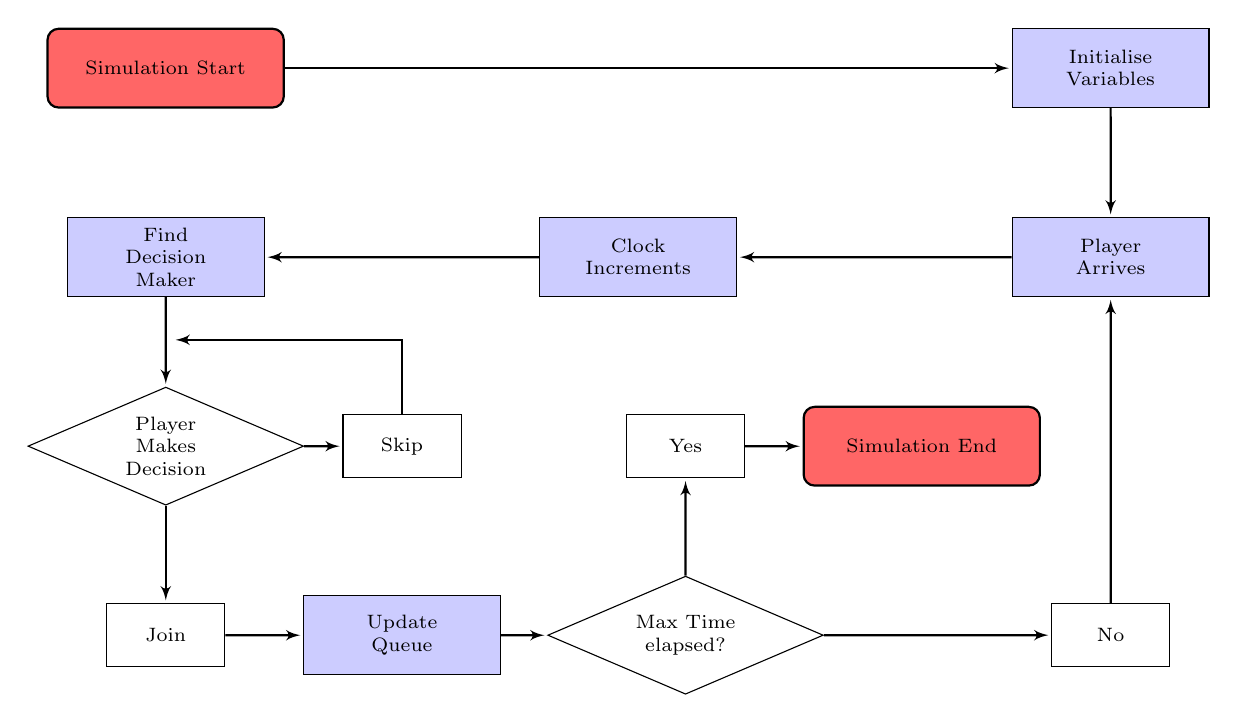
\begin{tikzpicture}[scale=.6]
        \tikzstyle{every node} = [font=\scriptsize ]

        %%%%% Top Line %%%%%%

        \draw (0,0) node[Terminal] (A) {Simulation Start};
        \draw node[Process] at ($(A)+ (20,0)$) (B) {Initialise Variables};


        %%%%% Second Line %%%%%

        \draw node[Process] at ($(B)+ (0,-4)$) (C){Player Arrives};
        \draw node[Process] at ($(C)+ (-10,0)$) (D){Clock Increments};
        \draw node[Process] at ($(D)+ (-10,0)$) (E){Find Decision Maker};

        %%%%% Third Line %%%%%

        \draw node[Decision] at ($(E) + (0,-4)$) (F){};
        \node[text width=1.5cm,align=center] at (F) {Player Makes  Decision};
        \draw node[Result] at ($(F) + (5,0)$) (G){Skip};
        \draw node[Result] at ($(G) + (6,0)$) (H){Yes};
        \draw node[Terminal] at ($(H) + (5,0)$) (I){Simulation End};

        %%%%% Bottom Line %%%%%

        \draw node[Result] at ($(F)+ (0,-4)$) (J){Join};
        \draw node[Process] at ($(J) + (5,0)$) (K){Update Queue};
        \draw node[Decision] at ($(H) + (0,-4)$) (L){};
        \node[text width=1.5cm,align=center] at (L) {Max Time elapsed?};
        \draw node[Result] at ($(C) + (0,-8)$) (M){No};

        %%%%% Connecting Arrows %%%%%

        \draw [Arrow] (A) -- (B);
        \draw [Arrow] (B) -- (C);
        \draw [Arrow] (C) -- (D);
        \draw [Arrow] (D) -- (E);
        \draw [Arrow] (E) -- (F);
        \draw [Arrow] (F) -- (J);
        \draw [Arrow] (J) -- (K);
        \draw [Arrow] (K) -- (L);
        \draw [Arrow] (L) -- (M);
        \draw [Arrow] (M) -- (C);
        \draw [Arrow] (F) -- (G);
        \draw [Arrow] (L) -- (H);
        \draw [Arrow] (H) -- (I);

        \node[draw=none,fill=none] at ($(E)+ (0,-1.75)$) (dummy){};

        \path [left] (G.north) |- (dummy.east);

	\end{tikzpicture}

	\caption{Flow chart describing the simulation model}
	\label{fig:Simflow}
\end{figure}


Our simulation model will initialise with the system empty, however this would not represent the system it is attempting to represent. This is due to the fact that most systems do not begin with an empty queue (e.g. a GP surgery would already have appointments scheduled, which would represent players in a queue in the context of our model.) and the potential impact of this is discussed in \cite{cite022}. The behaviour we are investigating occurs when the system has reached steady state.  To ensure that we are getting results from the steady state of a model, we must first determine the length of time it takes before the results from the model become invariant with respect to time. In \cite{cite013}, a method is discussed for finding the correct length for a model to run before collecting results. The algorithm involves the simulation being run for an increasing amount of time, and the mean utilisation recorded along with the standard deviation. By plotting the mean utilisation, along with a 95\% confidence interval, we can see when the model reaches steady state conditions by seeing when the graph stabilises. In Fig.\ref{fig:Warm}, the mean and 95\% confidence interval of the results was plotted to find the parameters necessary to ensure the accuracy of our results. The three parameters which needed to be determined were the length of the simulation, the warm-up period and the number of times each instance would be repeated. . Using the method suggested previously, we concluded the we needed to run the model for 250 time units and a warm up period of 50 time units was required. The number of trials did not cause a large variation even for small number of repeats and we decided to go with 16.

%\begin{figure}[ht]
%
%        \begin{subfigure}[b]{0.3\textwidth}
%                \centering
%                \includegraphics[width = 4cm]{./Images/Run_time.pdf}
%                \caption{Run Time}
%                \label{fig:Run}
%        \end{subfigure}
%        \begin{subfigure}[b]{0.3\textwidth}
%                \centering
%                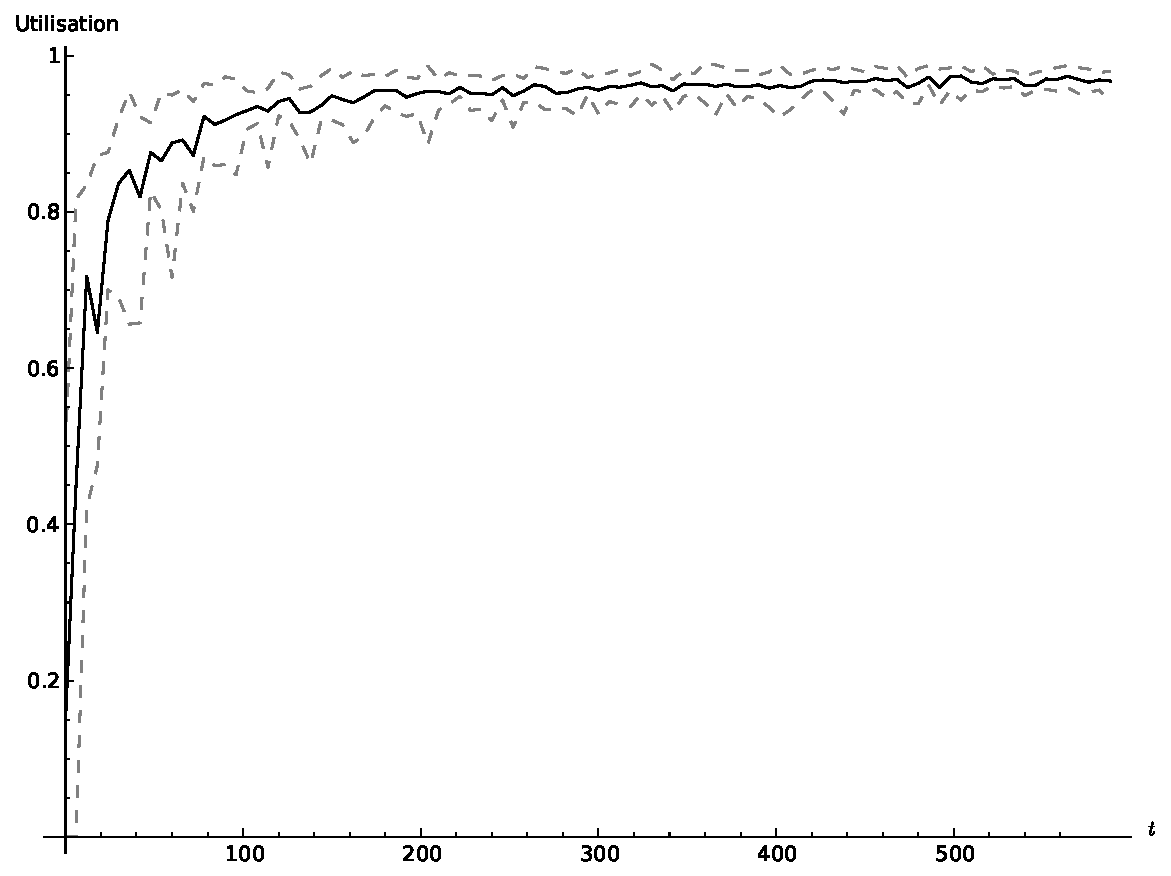
\includegraphics[width = 4cm]{./Images/Warm_up.pdf}
%                \caption{Warm-up time}
%                \label{fig:Warm}
%        \end{subfigure}
%        \begin{subfigure}[b]{0.3\textwidth}
%                \centering
%                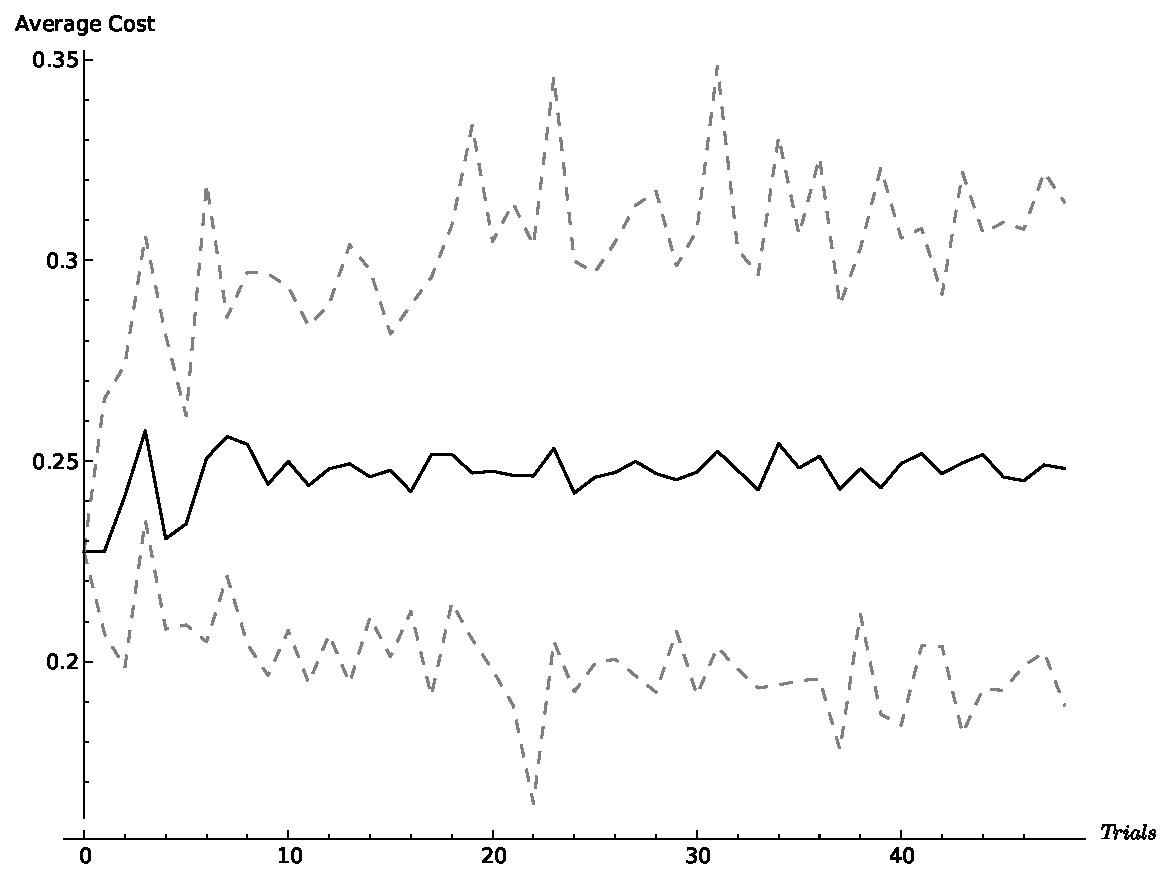
\includegraphics[width= 4cm]{./Images/Trials.pdf}
%                \caption{Trials}
%                \label{fig:Trials}
%        \end{subfigure}
%        \caption{Various graphs showing stabilisation of utilisation and cost as the simulation time increases }\label{fig:stable}
%\end{figure}

 To be able to effectively investigate larger scenarios, we started to use the Cardiff University supercomputer, Merlin \cite{web002}.The model is an example of embarrassingly parallel problem\cite{cite005}, due to the number of trials which enabled us to take advantage of the large number of cpu's available on Merlin\cite{cite007}.



%  \begin{figure}[ht]
%      \begin{center}
%          \begin{tabular}{ |c |c |c|}
%                                \hline
%            \multicolumn{3}{|c|}{Time taken in seconds}      \\ \hline
%            Original Model  & Improved algorithm & \% time taken  \\ \hline
%            35.7835  & 17.5425 &	49.02\\ \hline
%            25.0892  & 12.6983 & 	50.61\\ \hline
%            42.8013  & 19.9443 &	46.59\\ \hline
%            12.5448  & 5.8681  &	46.77\\ \hline
%          \end{tabular}
%
%          \caption{Comparison of the simulation model before and after implementing a new algorithm for finding the next decision}
%          \label{fig:Time}
%      \end{center}
%  \end{figure}



\section{Optimisation}

	The motivation for this paper is to study the effect that choice has on these particular systems, by using the Price of Anarchy as a measure of the inefficiency. To understand the impact of choice, we do not need the optimal social policy, but merely a good approximation to the optimal social policy. In \cite{cite023} a variety of heuristic methods are discussed, along with criteria for when a heuristic is applicable and what makes a good heuristic. We decided to use heuristic methods based on the conditions
    \begin{itemize}
    	\item{No exact method was known to find the optimal solution}
        \item{Although searching the solution space exhaustively would eventually yield the optimal solution, this proved to be far to computationally expensive }
    \end{itemize}

Based on these criteria, the following heuristic algorithms were tested.

We considered a variation on a local search heuristic, where after choosing our starting point as the selfish policy, we search a small area around this point exhaustively. If we find a better solution, we re-center our search space on the improved policy. One version of this algorithm did not change the search range (labeled search range \ref{fig:Solver_comp}), but there was an alternate version that if it did not find a better policy with the search space, it increased the range in which it searched (labeled variable search range \ref{fig:Solver_comp}). While this heuristic will eventually find the optimal policy (as the entire space of possible policies will eventually be searched) the method required a long time to run even small instances (even with the resources available described in chapter 3). As such the algorithm suffered a problem common to hill climbing heuristics, become locked into a local optima. By examining Fig. \ref{fig:Solver_comp} we can see that the performance of the algorithm was significantly worse due to the limited number of iterations we could run. The use of a similar hill-climbing heuristic within the context of a probabilistic model can be found in \cite{cite024}, including an examination of its use to find local optima.

 Another, simpler heuristic was investigated. A Random descent heuristic simply searches the solution space randomly, sometimes bound by conditions, but also completely unbound. While we experimented using a random walk which optimised each stations policy individually (labeled iterative \ref{fig:Solver_comp} ), it was found that this method was either similar, or at times worse than a completely random method. By again referring to Fig. \ref{fig:Solver_comp} we can see that this algorithm vastly out performed the local search algorithm.

%\begin{figure}[ht]
%    \begin{center}
%
%		\includegraphics[width=12cm]{Images/Solver_comp.pdf}
%		\caption{Comparison of the Local Search and Random Descent}
%		\label{fig:Solver_comp}
%    \end{center}
%\end{figure}


%%%%%%%%%%%%%%%%%%%%%%%%%%%%%%%%%%%%%%%%%%%%%%%%%%%%%%%%%%%%%%%%%%%%%%%%%%%%%%%%%%%%%%%%%%%%%%%%%%%

\section{Analytical Approximation}

	To reduce the computational cost of the investigations, we now propose an analytical approximation of the above model. For reasons that will become clear, we assume that despite the non-markovian nature of the decisions made by the players the actual inter arrival rate at each of the stations follows a Markovian Distribution \cite{cite014}. The arrival rate into each station is given by (\ref{eq:Arrival}). This formula is based on the dropout probability and arrival rate at the previous station.

\begin{equation}\label{eq:Arrival}
  \lambda_{i} = \lambda_{i-1}\times(1-p_{i-1}\times(1-\pi_{N}^{(i-1)}))
\end{equation}

 We also need to consider that fact that players will not dropout of the system if they balk from a particular queue. This is represented in (\ref{eq:Arrival}) by $(1 - \pi_{N}^{(i-1)})$ which only applies the probability of a player exiting the system to the players that do not balk. $\pi_{N}^{(i)}$ is the probability of there being $N$ players in the queue, where $N$ is the point at which players skip, either selfishly or due to a policy.
 We can then obtain a formula for the expected cost to a player moving through the system, which is expressed in \ref{eq:Expeccost}. The formula is a sum of the cost at each station, multiplied by the percentage of $\Lambda$ that arrives into station $j$

\begin{equation}\label{eq:Expeccost}
   C = \sum_{j=1}^{n}\frac{\lambda_{j} C_{j}}{\Lambda }
\end{equation}

We can approximate the cost to a player going through station $i$ by calculating the probability that station $i$ will have $m$ players in it\cite{cite018}. This probability is given by

\begin{equation}\label{eq:probcl}
  \pi_n = \frac{1}{n!}\left(\frac{\lambda}{\mu}\right)^{n}\pi_{0} \hspace{1cm} 0\leq n \leq c
\end{equation}

\begin{equation}\label{eq:probcm}
  \pi_n = \frac{1}{c^{n-c}c!}\left(\frac{\lambda}{\mu}\right)^{n}\pi_{0} \hspace{1cm} c< n \leq K
\end{equation}

where

\begin{equation}
\pi_{0} = \left[ \sum_{n=0}^{c-1} \frac{1}{n!} \left( \frac{\lambda}{\mu} \right)^{n}  + \sum_{n=c}^{K} \frac{1}{c^{n-c}c!} \left( \frac{\lambda}{\mu} \right)^{n} \right] ^{-1}
\end{equation}

Station $i$ is then in K+1 states given that there are $N$ players in the queue. Either the queue has less than c players(\ref{eq:probcl}), between c players and the maximum queue capacity K players(\ref{eq:probcm}) or the queue is full with K players in the system. By using these probabilities and the formula for expected cost(\ref{eq:expect}) we can calculate the $C$ given in (\ref{eq:Expeccost})

\begin{equation}\label{stationcost}
C_{i} = \pi_{N}^{(i)} \beta_{i} + \sum_{j=0}^{c_{i}} \frac{\pi_{j}^{(i)}}{\mu_{i}} + \sum_{j=c_{i}}^{N-1}\frac{ \pi_{j}^{(i)}(j+1)}{ \mu_{i} c_{i}}
\end{equation}

This is an analytical approximation and was verified by comparing it to the simulation model as can be seen in Fig.\ref{fig:Ana_comp}. The analytical model was a vast improvement in speed and efficiency over the simulation model. It allowed each possible policy to be evaluated and the expected cost per player to be approximated.a Searching the policy space exhaustively took less time than running a heuristic method.


%\begin{figure}[ht]
%    \begin{center}
%
%		\includegraphics[width=12cm]{Images/PoA_v_Demand_comparison_2S.pdf}
%		\caption{Comparison of the analytical model data to the simulation model for the case study}
%		\label{fig:Ana_comp}
%    \end{center}
%\end{figure}


An assumption made to compute this analytical approximation was that the arrival rate into any given station was Markovian. However, due to this assumption the analytical model may not always give such a close approximation to the simulation result [\ref{fig:Bad_Analyt}]. This is due the fact that the equations used in \cite{cite018} assume an $M/M/C/K$ queue, but the dropout probability causes our system to become a series of $G/M/C/K$ queues.


%\begin{figure}[ht]
%    \begin{center}
%
%		\includegraphics[width=12cm]{Images/Bad_Analyt.pdf}
%		\caption{Comparison of the analytical model data to the simulation model with a dropout probability}
%		\label{fig:Bad_Analyt}
%    \end{center}
%\end{figure}

Considering the case such that we have no probability of a customer leaving the system, the system as a whole exhibits Quasi-reversibility\cite{cite018} which means that the arrival and departure rate is time independent. Burke's theorem \cite{cite025} states that an $M/M/C$ queue with arrival rate $\lambda$ which is sampled from a poison distribution has the following properties.

\begin{itemize}
    	\item{The departure process is a Poisson process with rate parameter $\lambda$. }
        \item{At time t the number of customers in the queue is independent of the departure process prior to time $t$.}
    \end{itemize}

It is possible to obtain the optimal social policy for a single $M/M/1$ queue, called the Naor threshold \cite{cite026}. The result given describes the threshold at which players should balk from a single queue, and some preliminary results show that for no dropout probability and 1 server and each station, this does hold for our system.

%\begin{figure}[ht]
%    \begin{center}
%
%		\includegraphics[width=12cm]{Images/pdf_graphs.pdf}
%		\caption{Showing that the probability of a player entering each station approximates a Markov distribution }
%		\label{fig:Markovian}
%    \end{center}
%\end{figure}

%%%%%%%%%%%%%%%%%%%%%%%%%%%%%%%%%%%%%%%%%%%%%%%%%%%%%%%%%%%%%%%%%%%%%%%%%%%%%%%%%%%%%%%%%%%%%%%%




%    \begin{figure}[ht]
%    	\begin{center}
%
%        	\includegraphics[width=10cm]{Images/Varying_demand.pdf}
%            \caption{Varying the value of service at each station as demand increases}
%            \label{fig:Demandparam}
%      \end{center}
%	\end{figure}

%    \begin{figure}[ht]
%    	\begin{center}
%
%        	\includegraphics[width=10cm]{Images/Varying_Parameters_EXT.pdf}
%            \caption{Varying the exit parameters for different balking costs}
%            \label{fig:EXTparam}
%      \end{center}
%	\end{figure}


\break


%%%%%%%%%%%%%%%%%%%%%%%%%%%%%%%%%%%%%%%%%%%%%%%%%%%%%%%%%


\section{Conclusions and further work}

	We have considered a hierarchical system in both selfish and social conditions. By looking at the price of Anarchy in a series of $M|M|C$ queues we can conclude

    \begin{itemize}
    	\item{There exists a dropout probability such that the negative impact due to choice is minimised. }
        \item{The hierarchical structure contributes to the Price of Anarchy. However the dropout probability can alter and disguise this effect on the system.}
        \item{Increasing the cost to a player balking increases the Price of Anarchy.}
    \end{itemize}

There is much debate whether or not choice is beneficial to a given system. An example of this is within the NHS, and there are points of view that suggest that patients are happier with some element of choice \cite{cite017} and some that state that it is better to have a controlling element \cite{cite016}. However, from a strictly academic point of view, this paper has shown that by designing a system in certain ways we can minimises the negative impact due to individual behaviour. By only having a certain proportion of players remain within the system after completing service, the Price of Anarchy is minimised. The cost to a player for skipping a queue can be equated to how much service at a particular station is worth to players. By changing the worth of service at a station it is possible to increase and decrease the Price of Anarchy.It has also been shown that having a hierarchical structure within the queueing system can affect the Price of Anarchy, but is dependent on the dropout probability at previous stations. Usually it is advantageous to have a social policy that dictates players balk from queues earlier than they would under selfish conditions. However, If there is a large enough dropout probability, it can be better for players join a queue with more players ahead of them than under selfish conditions.

  Further work on this project would include some technical aspects, such as improving the performence of the simulation model. In this system, the arrival and service times are sampled from a markovian distribution, and it may yield some insights into the behaviour of the system if we consider other distributions. As in \cite{cite010}, altering the amount of information given to players such as the exit probability at each queue would give greater insights into how that probability affects the Price of Anarchy. Giving less information to the players and making the system unobservable could be compared to the existing system to show how this affected player choice.
    This model can be changed very slightly to give a completely different system. Instead of making a skip or a join decision upon entering a particular queue the player makes one decision upon entering the system, which queue to join inititally. This one change completely alters the structure of the policy and  the approximation of the cost of joining at a particular point. The investigation of this model, particularly with the focus on the new structure of the policy would be the primary focus of any future work.

\pagebreak
\bibliographystyle{plain}
\footnotesize{\bibliography{bibliography}}

\end{document}
